\documentclass{UoYCSproject}
% Preamble
\usepackage{bookmark}

% Pseudocode
\usepackage{algpseudocode}
\usepackage{algorithm}
\usepackage{amsmath}

% Table
\usepackage{booktabs}
\usepackage[normalem]{ulem}
\useunder{\uline}{\ul}{}

% referencing
\usepackage[backend=biber]{biblatex}
\addbibresource{references.bib}
\usepackage{url}     % This is needed for IEEE referencing

% Images
\usepackage{graphicx}
\graphicspath{ {../images/} }

% Title Page
\author{Babar Khan}
\title{Predicting Memorable Regions Of Images}
\date{2023-April}
\protect\supervisor{Adrian Bors}
\SWE

% Document
\begin{document}
\pagenumbering{roman}
\maketitle

\chapter{Abstract}
Memorability is known to be an intrinsic property of images \cite{Isola2011,IsolaParikhTorralbaOliva2011}, and in this report I investigate the potential of three different image to image models to learn to predict memorable regions of images, these are autoencoders, GANs, and diffusion models. I do this by performing supervised training with the image to memorability maps present in the VISCHEMA Plus dataset \cite{VischemaPaper}. This is useful to a large number of industries, particularly marketing and education. Recent research has found that diffusion models are able to synthesise images with greater image sample quality than GANs \cite{dhariwal2021diffusion}, and recent diffusion models have seen immense commercial success where GANs never did \cite{ramesh2022hierarchical, saharia2022photorealistic}. I investigate if that same success can be found in this domain.
 
\chapter{Executive Summary}


% state the aim of the reported work,
% motivate the work,
% state methods used,
% state results found, and
% highlight any legal, social, ethical, professional, and commercial issues as appropriate to the topic of study (if none, then this should be explicitly stated).


\textbf{Research Purpose, Motivation, and Methodology}

%The purpose of the research (what's it about and why's that important)
I investigate a range of deep conditional image to image generative models and evaluate their success when learning a mapping of images to memorable regions across three different experiments. 
% motivate the work
As shown in \cite{Isola2011,IsolaParikhTorralbaOliva2011}
% DOUBLE CHECK THOSE SOURCES
memorability is an intrinsic property of images, just like saliency, composition, or attractiveness, we can hopefully use these models to design images that are more memorable. This has far reaching uses, from marketing, education, entertainment, and more. The memorability of an image is intuitively affected by its surroundings, so being able to predict the memorability of a region within a image is extremely useful to the iterative design process within these professions.  
%The methodology (how you carried out the research)
These models were trained through supervised learning of image to VMS pairs in the training portion of the VISCHEMA Plus dataset. I compare these models using a set of defined requirements, including the L1 loss of their predicted memorability maps across the validation portion of the dataset, the qualitative quality of the predictions, and the time to train and evaluate the models.
%The key research findings (what answers you found)

\textbf{Findings and Implications}

Using a basic UNet Autoencoder I was able to generate semi accurate VMS maps that had low L1 losses of \(\sim 0.132\), but failed when examined qualitatively due to their tendency to smooth out the blocky VMS shape into circles.
Using a modified pix2pix GAN model \cite{isola2018imagetoimage} I was able to generate very accurate VMS maps, maintaining the blocky shape of the regions, and achieving a mean L1 loss of \(\sim 0.0740\). Generally, these models took longer to train than my autoencoder models.
Diffusion models took the longest to train, and while they have been shown capable of producing high quality images \cite{ramesh2022hierarchical, saharia2022photorealistic}, the training loop requires a large amount of computational resources, making it difficult to fine tune in a reasonable time. My best model was able to achieve an L1 loss of (Final Diffusion Loss), but due to computational restraints I was unable to run a large hyperparameter search and my results leave room for improvement.
% FILL IN FINAL DIFFUSION LOSS

%The implications of these findings (what these answers mean)
I show that using a GAN model we are able to predict memorable image regions with great accuracy. I believe this has many useful applications across many different industries, it will allow creators a more informed opinion on which regions of their images are memorable, using this tool to iteratively improve their image memorability. Hopefully in future work good parameters can be found that allow diffusion models to work with lower noise steps and to produce higher accuracy results.

% Ethical concerns
\textbf{Ethical Concerns}

I see no ethical concerns with the work presented in this report. I use the VISCHEMA Plus dataset, gathered by allowing human participants to indicate which image regions are memorable to them. I do not believe that any harm will come to said participants by carrying out this project as all data used is anonymised; the only data that Akagunduz et al. published about their subjects was that they attended the University of York, this is not enough information to identify them. As discussed by Dastin \cite{dastin_2018} and Najibi \cite{najibi_2020} it is important to train on a dataset without bias, as this bias can manifest within your learned models. It is impossible for us to know if the participating students represented a diverse subset of the population. As such, if we assume the worst case, that all of them are biased towards the same output, this would manifest itself within the data as the same regions being memorable. If our models were to train on this data then it would predict the same biased regions, and I see no way in which this could cause harm, it would simply predict unmemorable regions.

There are no legal, social, or professional concerns with the work conducted in this project.

\chapter{Introduction}

% This should be 2 pages
% need to define well what i am doing

\textbf{Background}

We are constantly surrounded by imagery, we see it: on the way to work, on the internet, on TV, in stores, and every time we use our eyes. Some images stick out more than others, we see hundreds, if not thousands, of images a day, and yet culturally and individually we all remember similar ones. Due to cultural significance an image can become memorable. The 2015 dress \cite{BBCDress2015}, a country's flag, or the 1932 image “lunch atop a skyscraper” \cite{gambino_2012}, come to mind. I argue that the memorability of such images is tied to the culture surrounding them, not necessarily due to intrinsic properties within. The focus of this research is on the intrinsic properties within an image that make it memorable to an individual, akin to seeing an advert on a bus and then later recognising the same advert online.
%How do we measure the memorability of an image
% What work has shown independence of memorability from viewer?
% Isola et al in 2011
% Vischema dataset experiments
It has been shown that the memorability of an image is an intrinsic property, independent from the viewer \cite{Isola2011, IsolaParikhTorralbaOliva2011, ICCV15_Khosla, isola2014memorability}, This is taken further by Akagunduz et al. \cite{VischemaPaper} where, in a similar experiment, they measure which regions of images are memorable and find that these regions are consistent among participants.

\textbf{Motivation}

% Why do we want to do this
%Why do we want to create a memorable image
%How does this research help to create a memorable image

Creating memorable images is the goal of many industries, in education you want to create learning resources remembered by students, in marketing, adverts remembered by customers, and in movies or TV, scenes remembered by audiences. Its been shown that with great accuracy we can train a deep neural network to predict the memorability score of an image \cite{Isola2011, IsolaParikhTorralbaOliva2011, ICCV15_Khosla, isola2014memorability},
% Double check sources
that is, assign a float in the range of [0,1] to an image, with a higher score indicating higher memorability. But I propose that the memorability of an object within an image may be independent from the memorability of that object on its own. For example, an advert's memorability may not be equal to the memorability when seen in an environment such as on the side of a bus or building, in these cases the advert competes with everything else the viewer observes. This gives great importance to the examination of image region memorability, hypothetically a person wanting to create a memorable image could render their image on the side of a bus or building digitally, and test the memorable regions of that rendered image. They could then iteratively modify and examine their image until it is the most memorable region of the scene.

%What are my goals

To create a model that does this is an incredibly difficult task, success has been found in semantic image segmentation \cite{wang2023internimage} and I believe that this task is a continuous variation of it. My motivation with this work is to both gain a deeper understanding of image memorability, and to gain experience using image to image deep convolutional networks. I want to create an accurate mapping from image to memorability maps. As I am using the VISCHEMA dataset in a supervised learning environment, I can measure the accuracy of my models as the mean absolute difference between my network output and the ground truth label present in the dataset.

\textbf{Report Structure}

This report is organised as follows: Chapter 4 discusses existing literature in image memorability, Chapter 5 discusses the project methodology, I describe available deep learning datasets and existing image to image models, Chapter 6 details my experiments and results, and Chapter 7 my conclusion, where I discuss the implications of my findings and possibilities for future work.    

\chapter{Literature Review}

% This should be 6-8 pages long

\textbf{Memorability}

% Roy Brener An experimental investigation of memory span
% Subjects were presented with units of varying length and were asked to recall them
% The unit could be a sentence, a digit, a geometric shape, etc
% It was found that people are not very good at remembering nonsense sylables or sentences but are much better at remembering digits, consonants, and colours. Remembering geometric designs is placed somewhere in the middle.
% This would seem to indicate that people are not very good at recalling images, however in Nickerson's work we can see that subjects are extremely good at recognising images. 

In Breners work \cite{BrenerMemorySpan} subjects' abilities to remember a series of units was tested, with units defined based on the test performed, 
\begin{quote}
    In the digit test, for example, each digit was a unit; in the sentence test each sentence was a unit, etc. ... Each nonsense syllable constituted a unit ... Each consonant constituted a unit ... Each [geometric] design constituted a unit. \cite[p.468]{BrenerMemorySpan}
\end{quote}

Each unit was presented to participants on a piece of card, one card was shown every two seconds, and at the end of the series of cards participants would have to repeat the series to the experimenter. If a participant repeated all units correctly then the length of the series would increase, otherwise it would decrease. Once a subject could answer the entire series correctly, every other series length was tested. It was found that people are not very good at remembering nonsense syllables or sentences but are much better at remembering digits, consonants, and colours. Remembering geometric designs is placed somewhere in the middle. This is of interest because it is very similar to our investigation into what aspects make images memorable. Brener was interested in consonants, colours, geometric designs, and other units, and his finding that different units can be significantly harder or easier to remember is useful to us. If we swap out units for image properties such as texture, contrast, saturation etc, or even more abstract features that a CNN may recognise, then it should be possible to find how memorability is impacted by these. 
 

% R. Nickerson Short-term memory for complex meaningful visual configurations 1965
% Subjects are shown new and old photos and they have to identify if the photo is new or old
% P(Ro/So) = ~0.9
% 95% of all responses were correct
% subjects were more likely to correctly identify a photo as new than they were to correctly identify a photo as old
% Shown 1 image at a time with 50% chance of being old and 50% chance of being new
% 
The mean score of 5.31 found for geometric designs seems to indicate that people are not great at recalling images, however in Nickerson's extremely influential work \cite{NickersonShortTermMemory} we can see the opposite, subjects are found to be extremely good at recognising previously seen images. Nickerson found that subjects shown a series of images are, with great accuracy, able to recall if the photo is one they have seen before or not. An item is referred to as 'new on its first occurrence and old on its second occurrence'\cite[p.156]{NickersonShortTermMemory}, it was found that subjects shown one image at a time, each with equal chance of being old or new, are able to correctly distinguish them with 95\% accuracy. Nickerson's experiment is very different to Brener's, in the former a subjects ability to recognise an image is tested, where as in the latter subjects abilities to recall is tested. Nickerson laid the groundwork for the memorability game that all experiments described ahead are based on and adapt.  

Like in \cite{NickersonShortTermMemory}, Shepard's work in \cite{ShepardRecognition} also found that subjects are able to distinguish with great accuracy new and old images, the mean percentage of images correctly identified was 99.7\% after a delay of 2 hours, 92.0\% after a delay of 3 days. 87.0\% after a delay of 7 days, and 57.7\% after a delay of 120 days. The introduction of a delay into the memorability game allows us to see that regardless of whether the image is in our short-term memory (2 hour delay) or our long-term memory (3-120 days) subjects are able to correctly identify an incredible amount of images. This 

% L. Standing. Learning 10,000 pictures. In Quarterly Journal of Experimental Psychology, 1973
% ## What is the goal of this paper ##
% Memory capacity and retrieval of pictures and words
% it shows that the capacity for memory of pictures is almost limitless, when measured under appropriate conditions. 
% People are able to recall images incredibly well  
% ## What are its limitations ##
% The experiments don't have many people involved Experment 2 only has 2 subjects and experiment 4, 4.
% He tested normal and vivid pictures
%------------
Standing built on the work of Nickerson, Shepard, and Brener in \cite{standing10000pictures}. Four experiments were ran which tested memory capacity and retrieval speed for pictures and words, I am interested in the performance related to pictures specifically. He found that, when measured under testing conditions, the capacity for image recognition from memory is almost limitless. In Standing's first experiment he tested 'normal' and 'vivid' images. He describes 'normal' images as those that 'may be characterized as resembling a highly variegated collection of competent snapshots'\cite[p.208]{standing10000pictures}, and 'vivid' images are described as 'striking pictures ... with definitely interesting subject matter'\cite[p.208]{standing10000pictures}. Much like how in Brener's work \cite{BrenerMemorySpan} the memorability of an object was variable based on what classification of unit was tested, this work shows that on an even more specific level, the classification of the image into normal or vivid, has an impact on subjects' memory, Standing found that the vivid images were more likely to be remembered by subjects.


% F. Brady, T. Konkle, G. A. Alvarez, and A. Oliva. Visual long-term memory has a massive storage capacity for object details. In Proceedings of the National Academy of Sciences, 2008
% This is about how much detail is required to remember an image, rather than if you can just remember it or not
% Are you truly only able to store the gist of items in your long term memory, or are we capable of more?
% It is shown that people are able to store far more information than just the gist in their long term memory, we are able to store fine grained details
% this builds directly onto the world of Standing in 1973
%------------

Lots of work has been done to further build on that of Standing, Nickerson, Brener et al. Brady et al. \cite{brady2008visual} performed research into how much information is retained in long term memory and found that subjects are able to remember not just the gist of an image, but also fine grain information such as the state of objects within an image, and that they are able to distinguish between variants of objects shown in images. An example shown was an abacus in two different states, 13/14 subjects were able to distinguish which one they had seen before.

% D. A. Brown, I. Neath, and N. Chater. A temporal ratio model of memory. Psych. Review, 2007.
%An exploration to the extend to which common retrieval princples apply to human memory over short and long timescales
% Traces of items are represented in memory partyly in terms of how long ago they were observed
% Similar mechanisms govern retrieval from memory over many different timescales

In \cite{KonkleDistinct} Konkle et al. build further on the work in \cite{standing10000pictures, brady2008visual} by studying the impact that categorical distinctness has on memorability. This was tested by creating a dataset of images composed of categories such as tables, cameras, and bread etc. Each category had between 1 and 16 images, and a standard memory game like those performed in \cite{NickersonShortTermMemory, standing10000pictures, brady2008visual}
% check which other memory tests this matches
was performed. The percentage correctly identified was found to decrease as the number of images within a category increased, from this we can see that categorically distinct images are more likely to be remembered. 

Groundbreaking studies by Isola et al. \cite{Isola2011, IsolaParikhTorralbaOliva2011} were performed with the goal of identifying a collection of visual attributes that make images memorable, and to use those to predict the memorability of an image.
They performed a memorability game similar to the work described above and used this to assign a memorability score to each image, their work finds that image memorability is consistent among participants and that even after seeing potentially hundreds of images, participants can correctly recognise a previously seen image.
It was found that properties such as mean saturation, and the log number of objects, have less impact on the memorability score than object statistics.  Categories such as: person, person sitting, and floor, were most helpful image memorability. The categories: sky, tree, and mountain, were least helpful.
Their approach was unfortunately limited by the fact that the object statistics were annotated by hand, this would both make automating the process of determining image memorability impossible, and limit them from finding any abstract properties that helped/hindered memorability. Nevertheless, this work is incredibly influential and most memorability work going forward has built on this.

Khosla et al. \cite{NIPS12_Khosla} built on the work in \cite{Isola2011, IsolaParikhTorralbaOliva2011} by, instead of determining memorability of an entire image, creating a model that discovers memorability maps of individual images without human annotation. These memorability maps are able to distinguish which areas of an image are remembered, forgotten, or hallucinated. These memorability maps are binary vector encodings of the external and internal representations, $v_j$ and $\tilde{v}_j$ respectively, each with indexes for every annotated object category. The external representation refers to the ground truth image, where as the internal representation refers to the image that a person may store in their memory. They describe the noisy process of external to internal representation, and how some objects are forgotten, remembered, or hallucinated. The distance between $v_j$ and $\tilde{v}_j$ is inversely proportional the memorability of an image. By testing the effect of gradient, colour, texture, saliency, shape, and semantics on image ,memorability they are able to compute memorability map images. Their approach, similar to Isola et al. in \cite{Isola2011, IsolaParikhTorralbaOliva2011}, is limited by the arbitrarily picked list of features that define memorability.  

Further work by Khosla et al. in \cite{ICCV15_Khosla} showed how you can use deep learning to learn to predict the memorability of an image using supervised learning of image and memorability pairs. They conduct a large scale memorability game experiment across 60,000 images, using a similar protocol to \cite{isola2014memorability}, and build a convolutional neural network, MemNet, capable of predicting memorability with a rank correlation of 0.64.  

\textbf{Literature Conclusion}

There has been lots of work on human memorability but it wasn't until recently that work on determining image memorability automatically had been done. The work by Isola et al. \cite{Isola2011,IsolaParikhTorralbaOliva2011} and Khosla et al. \cite{ICCV15_Khosla} represents the current state of the art in image memorability, using deep learning to automatically determine the memorability of images.

\chapter{Methodology}

% This should be from a theoretical perspective
% No need for specific values, just describe what I plan on doing

In this chapter I describe the methodology of my project, the requirements for success, an overview of state of the art probabilistic models used to synthesise images, and considerations for the design options and implementation environments. 

During this project I followed a Waterfall method, a sequential development process where each step iteratively builds on and requires the last. A prominent criticism of the Waterfall method is its lack of flexibility, and that criticism is why modern software development tends to use an Agile design method, however due to the fact that the requirements of this project are known beforehand, the Waterfall method is more appropriate. There are 4 relevant Waterfall steps that I will follow and that are described in figure \ref{fig:waterfall method}. These are: The requirements capture, the design, the implementation, and the testing.

\begin{figure}[ht]
    \centering
    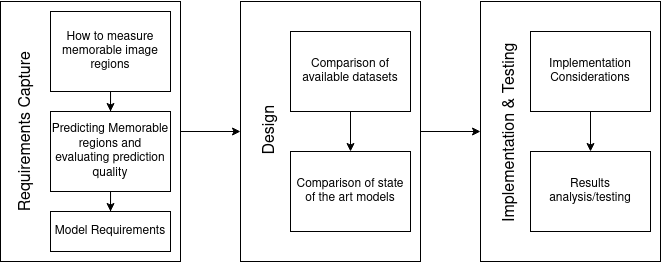
\includegraphics[width=\linewidth]{Waterfall Model} % CHANGE THIS
    \caption{Waterfall Method Steps}
    \label{fig:waterfall method}
\end{figure}

\textbf{How to measure memorable regions of images}

There are two approaches to measuring the memorable regions of an image. Both approaches have subjects try to remember previously seen images, like in
% Memorability experiments
The approaches differ in their execution of the memorability game. Firstly, like in LaMem \cite{ICCV15_Khosla}, you split an image into many regions, and use a model designed to predict the memorability of an image to predict the memorability of that region, then, compose these memorability, region pairs into a memorability map. 
Alternatively, like in VISCHEMA \cite{VischemaPaper}, when a user indicates that they remember an image, allow them to mark the region of the image that caused them to remember it. 
In either case the result is the same, a distribution of image, memorability map pairs in which supervised learning can occur on.

\textbf{Predicting memorable regions and evaluating prediction quality}

Assuming that we have a dataset of image, memorability map pairs as described above, then we can use an image to image deep convolutional model to learn a mapping from an image to its corresponding memorability map. 
There are many image to image models that exist, but fundamentally we can abstract the model as a function of an image, $I$, because of this we can evaluate each model across the same requirements. 
Given an image the model needs to predict what the corresponding memorability map looks like.
We can evaluate the quality of these solutions in a number of ways. The L1 and L2 loss can describe the absolute and mean square error between two equally sized images. We can also compare the outputs of our models quantitatively, do the predicted outputs look similar to the inputs. Its possible that our models could learn to predict something simple, like a single shade of green, entirely black images, or just noise, in this case the outputted labels would be worthless. We can evaluate this behaviour though qualitative analysis of the output images. Execution time is also important, I propose that this system can be used by creatives to iteratively improve their images, if it takes too long to evaluate a single image on modern hardware then it is less useful than a similar performing model that performs much faster.

\textbf{Model Requirements}

In figure \ref{tab:RequirementCaptureTable} I describe the requirements that each probabilistic model will be compared against. A model will be considered unsuccessful if it does not meet every requirement in the "must" section, and will be considered somewhat successful if it meets all of those in the "must" section but not all of those in the "should" section.

\begin{table}[ht]
    \begin{tabular}{p{0.1\linewidth} p{0.6\linewidth} p{0.3\linewidth}}
    \toprule
    ID  & Description & Kind \\ \midrule
    \multicolumn{3}{l}{{Must}} \\
    \hline \\
    1.1 & The implementation of the model should be able to take an image from the dataset as input. & Functional \\
    1.2 & Given an image, the model must output an image the same size as the corresponding memorability map. & Functional \\
    1.3 & The average loss of the model output given an image, and the corresponding label, should be low. & Non-Functional \\
    1.4 & When outputs of our model are compared qualitatively with the corresponding label they should look similar. & Non-Functional \\
    \hline \\
    \multicolumn{3}{l}{{Should}} \\
    \hline \\
    2.1 & The implementation of the model should evaluate images quickly; it should not take longer to than a second to generate a memorability map. & Non-Functional \\
     &  &  \\ \bottomrule
    \end{tabular}
    \caption{Probabilistic Model Requirements Table}
    \label{tab:RequirementCaptureTable}
\end{table}

\textbf{Comparison of available datasets}

The two dataset options I have considered are LaMem \cite{ICCV15_Khosla} and VISCHEMA \cite{VischemaPaper}. 
LaMem contains 60,000 annotated image and memorability pairs. Memorability is measured as a continuous value in the range [0,1] where a higher value indicates that the image is more memorable. They then train a CNN to predict the memorability of an image, resize their images, and pass overlapping regions of the image into their CNN. The generated memorability maps are tested for accuracy by adjusting the original images to de-emphasise the regions indicated as memorable. These adjusted images are then tested using the original memorability game used to create the dataset.
VISCHEMA is a significantly smaller dataset, containing around 1600 images, memorability map pairs in the VISCHEMA Plus version. Their experiment differs from that of Khosla et al., they ask participants to memorize a set of images, and then during a test phase rate how well they remember each image and to select the regions that made them remember it. In order to predict memorability the network output utilises fully connected layers which I believe is unnecessary, and may even hurt performance. More modern computer vision network structures, such as those in \cite{ronneberger2015unet, goodfellow2014generative, ho2020denoising, isola2018imagetoimage, saharia2022palette}, use fully convolutional networks. These maintain spatial locality which allows them to generalise better.

The use of either of these comes with drawbacks, LaMem is a much larger dataset, containing 60,000 images compared to the 1,600 images in VISCHEMA Plus, this significant increase should allow any deep learning models to generalise far more easily. Unfortunately I am not entirely convinced of their methodology for generating memorability maps, the memorability of an image may not be equal to that of an image within another image. That is to say, the environment in which we see an image, intuitively, may have some impact on the memorability of it. In the latter, 
When gathering the VISCHEMA Plus dataset  Akagunduz et al. successfully measure the memorable regions of images, rather than a score per image which I believe to be more robust. Unfortunately, their dataset is very small, which means that more care would need to be taken to not cause our models to overfit. After evaluating both datasets I have chosen to use the VISCHEMA Plus dataset. 

\textbf{Comparison of state of the art models}

I will create and evaluate a range of deep convolutional image to image models that learn a mapping of VISCHEMA Plus images to their corresponding VMS labels. Our models will all be evaluated against the requirements detailed in \ref{tab:RequirementCaptureTable}. State of the art models would include, autoencoders, GANs, and diffusion models, as the three of them produce images in different ways I see value in comparing their performance in the same task. I will run three experiments where I train a UNet autoencoder, a GAN, and a diffusion model to produce a VMS label given an image from the dataset. I hope to be able to find the strengths and weaknesses of each of these systems. For each model I will experiment with network parameters and training hyperparameters to fine tune models that produce the best output.

In each experiment I will automate a system that: tests the effectiveness of different numbers of layers and channels in each network, varies the normalisation method, optimisation function, learning rate, and batch size to find the best training environment and model parameters. It is not be feasible to test every combination of these variables, thus I will employ a strategy where I test every variation of a single parameter/hyperparameter while keeping the rest constant. I will start each model with an estimation of good parameters, then iterate through each individual parameter, varying only that one and measuring the impact on performance. After testing all variations of a single parameter, I will pick the one that gave the highest score and move onto the next parameter. This will bring the size our search space down by an order of magnitude, however we will not be exploring the entire search space and will potentially miss out on good models. 

Due to the long training and evaluation time of diffusion models I plan on performing a smaller parameter/hyperparameter search for those, I hope to still achieve good results, but due to computational and time restrictions I will not be able to experiment as much as I want with them.
% TALK ABOUT DIFFUSION MODELS TAKING A LONG TIME TO TRAIN AND THUS GETTING LESS TESTING HERE

\textbf{UNet Autoencoders}

The autoencoder model is composed of 3 parts, an encoder, a bottleneck, and a decoder, these are typically used for compression. The U-Net \cite{ronneberger2015unet} is a variation of an autoencoder which has found great success in semantic image segmentation within the medical field. This architecture is the backbone of many image to image models \cite{isola2018imagetoimage,saharia2022palette,dhariwal2021diffusion}, and has seen many extensions \cite{zhou2020unet, Qin_2020}. A Diagram of the model can be seen in figure \ref{fig:autoencoderDiagram}, the model is composed of two blocks, an encoder and a decoder. 
The encoder, composed of convolutional filters, takes the full sized image and compresses it into a latent space vector.
Every layer in the encoder halves the resolution of the image and increases the number of channels, the decreasing resolution allows the model to capture image components at different scales. 
In the higher resolution layers the convolutional filters are able to see fine grain features, for example, the leaves in a tree. In the lower resolution layers convolution filters are able to see more coarse features, for example, at the deepest layer of the same image as above a forest of trees. 
The decoder then takes that latent space vector and uses up-convolution to create an output image. 
As the image is passed back through the decoder the opposite happens, the up-convolution layers increase the image resolution and decrease the number of channels. This allows the model to build the output image starting with very coarse details and then at the latter layers fine grain details.
The network makes use of residual skip connections, these allow the model to preserve encoding features from the encoder layers in the decoding stages, with these the model performs significantly better. These encoding features are concatenated directly onto the input at the opposite decoding layer. 

\begin{figure}[ht]
    \centering
    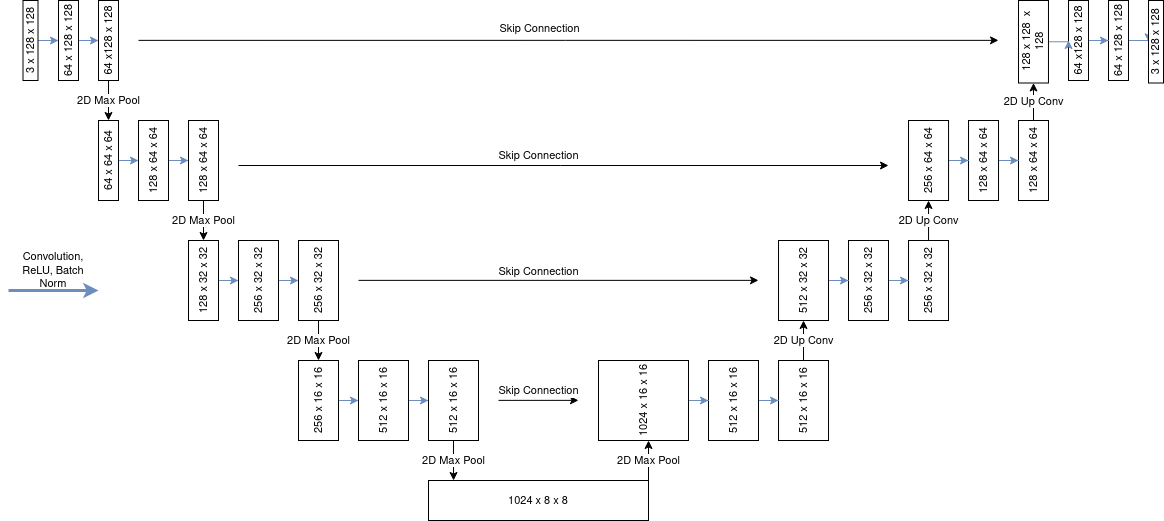
\includegraphics[width=\linewidth]{UNet Diagram}
    \caption{UNet Autoencoder Diagram}
    \label{fig:autoencoderDiagram}
\end{figure}

If we consider an image $ I $, a 3D matrix with width $ w_I $, height $ h_I $, and depth $ c_I $ and a corresponding label $ L $ to be a 3D matrix with width $ w_L $, height $ h_L $, and depth $ c_L $. Then an autoencoder works by taking image $ I $ and producing an output with dimensions equal to $ L $. We will call the ground truth label $ L_{real} $ and the autoencoder output $ L_{pred} $. As this is a regression problem there are a couple of options for loss functions. Firstly the Squared Elucidean norm, also known as MSE loss, this is effectively the distance between our prediction and ground truth label squared. The second option is the L1 loss, or the mean absolute error loss, this measures the absolute difference between our prediction and the ground truth label.
Because the L1 loss does not contain any square numbers I will choose to use it over the MSE loss, this should hopefully contribute to the prevention of the exploding gradients problem. Our Loss function is described in equation \ref{eqn:UNet Loss}

\begin{equation}
    \label{eqn:UNet Loss}
    \texttt{UNet Loss} = \frac{1}{w \times h \times c} \sum_{i = 0}^{w_L} \sum_{j = 0}^{h_L} \sum_{k = 0}^{c_L}(L_{real}[i,j,k], L_{pred}[i,j,k] ) 
\end{equation}

This loss describes the average absolute difference between each corresponding pixel in the ground truth label and the predicted label. Each convolutional layer within the UNet has adjustable weights $w$ that can be adjusted to produce a better output. The training loop uses backpropagation of this loss to adjust the model weights. To adjust a given weight $w_j$ calculate $ \frac{\delta L}{\delta w_j} $ and use gradient descent to adjust it. Please see algorithm \ref{ALG:Autoencoder} for the full training loop.

\begin{algorithm}
\caption{UNet Autoencoder Training Strategy}\label{ALG:Autoencoder}
\begin{algorithmic}[1]
\For{$\texttt{every epoch}$}
\For{$I, L_{real} \texttt{ in training dataloader}$}
\State
\State $L_{pred} = model(I)$
\State $loss = L1( L_{pred}, L_{real} ) $
\State $\texttt{Update weights of model with backpropagation}$
\State
\EndFor
\EndFor
\end{algorithmic}
\end{algorithm}

\textbf{Generative Adversarial Networks}

% presented by ian goodfellow and is composed of a generaor and a discriminator

The Generative Adversarial Network is an image synthesis model described by Goodfellow et al \cite{goodfellow2014generative}. In this model there are two adversarial networks, a generator, $ G $, and a discriminator, $ D $. I will describe a ground truth image as real, and one created by the generator as fake. The goal of the generator is to, given a latent space vector $ z $, produce an image that the discriminator thinks is real. The goal of the discriminator is to take an image, either real or fake, and predict which it is. In its vanilla form the loss of each network is relative to the performance of the other making it impossible to see if the networks have converged. The loss function described in \cite{goodfellow2014generative} is a minimax game, where G is trying to maximise the probability of D making a mistake, and D is trying to minimise it. More formally: The loss function of G is such that it is trying to maximise equation \ref{eqn:Vanilla Generator Loss} and the loss function of D is such that it is trying to maximise equation \ref{eqn:Vanilla Discriminator Loss}. Conditional generative adversarial networks can create images using a latent space vector and a condition parameter. For example, the class of the image to produce, simply pass this parameter into both the generator and the discriminator. In this case the discriminator outputs the probability that $ L $ is real and that meets the condition parameter.

\begin{equation}
    \label{eqn:Vanilla Generator Loss}
    Loss_G = -logD (G(z)) 
\end{equation}

\begin{equation}
    \label{eqn:Vanilla Discriminator Loss}
    Loss_D = -[c \times logD(x) + (1-c) log (1 - D(x))] \\
\end{equation}

\[ c =
\begin{cases}
  1, & \text{if}\ real(x) \\
  0, & \text{otherwise}
\end{cases} \]

Lots of work has gone into making GAN models more stable and I will use these findings in my own models. Brock et al. find that when 'increasing the batch size by a factor of 8 ... models reach better final performance in fewer iterations, but become unstable and undergo complete training collapse'\cite[3]{brock2019large}.
%Because of this I will experiment with early stopping and low batch sizes.
In \cite{zhao2020differentiable} Shengyu et al. show that using differentiable augmentation on your images increases the quality of the outputted images. With a dataset with as few as 100 images they are able to produce high quality outputs.
% This is useful to us because the VISCHEMA plus dataset only has 1280 training images, which typically wouldn't train very well on a GAN.

% pix2pix is a conditional generative adversarial network that is used for style transfer, it uses the UNet autoencoder as a backbone. The generator takes an input of size 3xwxh and produces a label of size 3xwxh. The discriminator takes the concatenation of the image and either the real or fake label, 6xwxh and produces an nxm array of boolean values describing, with each boolean describing whether a patch of the label is real or fake. 

%I will train a conditional generative adversarial network to generate images of VMS maps given images from the VISCHEMA dataset. I will use an adapted pix2pix network \cite{isola2018imagetoimage}, making tweaks that I think will increase performance. 
Pix2pix by Isola et al.\cite{isola2018imagetoimage}, is an image-to-image conditional generative adversarial model based on the UNet \cite{ronneberger2015unet}, designed for style transfer. In this model the generator takes a conditional image and uses that to produce a label, $L_{pred}$, the discriminator takes the concatenation of $I$ along with a real or fake label, and produces a 2D array of boolean values with width $N$, and height, $M$. Each value describes whether the corresponding patch in the image is real or generated. The loss for each network is slightly different to those described in a vanilla GAN, the generator loss is described in equation \ref{eqn:Pix2pix Generator Loss} describing how well it can both trick the generator, and how closely the output matches the input. The discriminator loss is described in equation \ref{eqn:Pix2pix Discriminator Loss}, similar to equation \ref{eqn:Vanilla Discriminator Loss} describes how well D can predict an images distribution. The training strategy for this network is described in algorithm \ref{ALG:GAN}. Please see figure \ref{fig:patchGANDiagram} for a diagram of this model.

\begin{equation}
    \label{eqn:Pix2pix Generator Loss}
    \begin{split}
    Loss_G = & \frac{1}{NM} \sum_{i=0}^{N} \sum_{j=0}^{M} (D(L_{pred}, I)_{[i,j]} -1 )^2\\
           + & \frac{1}{w_Lh_Lc_L} \sum_{i=0}^{w_L} \sum_{j=0}^{h_L} \sum_{k=0}^{c_L} |L_{pred}[i,j,k] - L_{real}[i,j,k]|
    \end{split}    
\end{equation}

\begin{equation}
    \label{eqn:Pix2pix Discriminator Loss}
    Loss_D = \frac{1}{2NM} \sum_{i=0}^{N}  \sum_{j=0}^{M} ( (D(L_{fake}, I)[i,j] )^2 + (D(L_{real}, I)[i,j] - 1)^2)
\end{equation}

\begin{figure}[ht]
    \centering
    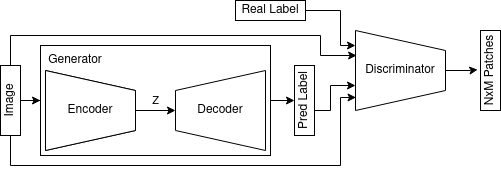
\includegraphics[width=\linewidth]{PatchGAN Diagram}
    \caption{Pix2pix Diagram}
    \label{fig:patchGANDiagram}
\end{figure}

\begin{algorithm}
    \caption{Pix2pix Training Strategy}\label{ALG:GAN}
    \begin{algorithmic}[1]
    \For{$\texttt{every epoch}$}
    \For{$I, L_{r} \texttt{ in training dataloader}$}
    \State
    \State $L_{f} = G(I)$
    \State
    \State $pred_{fake} = D(L_{f}, I) $
    \State $loss_G = MSE( pred_{fake}, 1 ) + L1(L_{f}, L_{r}) $
    \State $\texttt{Update weights of G with backpropagation}$
    \State
    \State $pred_{real} = D(L_{r}, I)$
    \State $loss_D = 0.5 \times  ( MSE( pred_{fake}, 0) + MSE( pred_{real}, 1) ) $
    \State $\texttt{Update weights of D with backpropagation}$
    \State
    \EndFor
    \EndFor
    \end{algorithmic}
\end{algorithm}
    

In \cite{arjovsky2017wasserstein} Arjovsky et al. introduce a GAN variant based on the Wasserstein distance of the output distribution and the image distribution, the benefit of this is that the Wasserstein distance is continuous and differentiable almost everywhere, reducing the risk of diminishing gradients. In this case the discriminator no longer outputs a value of $0|1$ and instead produces a continuous variable output, it is therefore renamed to a critic. In \cite{pix2pixwasserstein} Makow investigated the use of Wasserstein Distance in the pix2pix model but unfortunately found that it does not perform much better, however they were limited by their hardware and unable to perform a complete hyperparameter search. The lack of increase in performance is also likely due to the fact that in pix2pix the generator, not only tries to trick the discriminator, it is also trying to create images close to the ground truth labels, the second part of the loss function is continuous and thus that benefit of the Wasserstein distance is limited.

%I would still like to experiment with it as VISCHEMA plus is different from any dataset used in \cite{isola2018imagetoimage} and as Makow states they were unable to perform a complete hyperparameter search, meaning that its possible we could achieve greater results than vanilla pix2pix.
% I will be adapting the following PyTorch implementation \cite{PytorchPix2Pix} for my experiment. 



% https://www.youtube.com/watch?v=J97EM3Clyys
% https://github.com/mit-han-lab/data-efficient-gans/blob/master/DiffAugment-stylegan2-pytorch/DiffAugment_pytorch.py
% horizontal flips are a good application on the real images
% You could augment the real images -> this will cause the generator to learn to generate augments, this is bad for augments such as cutout
% You could augment the real images and the fake images when the discriminator sees them, the generator will have an easier time fooling the discriminator
% Solution: Augment real and fake images for the discriminator and the generator
% Need to be able to differentiate the augmentation so that we can update the generators weights using gradient descent
% How do we make our augmentations differentiable?
% We provide a torch tensor that represents the images as input, then we randomly sample parameters related to augmentation. e.g. translation amount or cutout coords. Apply this augmentation to the input tensor
% since it is all done using torch operations, the computational graph will be computed for these functions
% Kornia can do this for us.
% pass the augmentation module, kornia, into the discriminator. Apply augments on the input to the discriminator first but only when training 

%https://cs230.stanford.edu/projects_spring_2018/reports/8289943.pdf 


%Because these two loss values are relative to the performance of each other they can't be used to see if our generator has converged on a solution. Therefore it is necessary, at each epoch, to also compute the L1 loss of the fake labels and real labels across the training and the validation dataset, as these values are calculated independently of the discriminator. This will inform allow us to see if the generator is overfitting, underfitting, or training well. 



\textbf{Diffusion Models}

Diffusion based generative models work by learning to iteratively remove Gaussian noise from a sample T times until it produces an image from the training domain. The model was first proposed by Sohl-Dickstein et al. \cite{sohldickstein2015deep}, and has been further developed by Ho et al. \cite{ho2020denoising},  Dhariwal and Nichol \cite{dhariwal2021diffusion}, and Saharia et al. \cite{saharia2022palette}. They are a machine learning model that work through a forward diffusion process systematically destroying the structure in a data distribution, and the learning of a backwards process to restore the structure. The method uses a Markov chain to convert $ x_t $ into $ x_{t-1} $. Starting with $ x_T $, a sample of Gaussian noise, a generative Markov chain converts this into $ x_0 $, which is a sample from the target data distribution. Because the model only estimates small perturbations of noise, $ x_t $ given $ x_{t-1} $ , rather than an entire transformation from $ x_0 $ to $ x_T $, it is tractable to train. 

The DDPM is a diffusion model capable of producing high quality images and achieves state of the art FID scores across the CIFAR10 dataset \cite{ho2020denoising}. Dhariwal and Nichol \cite{dhariwal2021diffusion} show tweaks that allow for diffusion models to achieve state of the art FID scores across the ImageNet dataset and when used in combination with upsampling diffusion further improve FID scores. They do this by using improvements proposed in \cite{song2022denoising, nichol2021improved, song2021scorebased, brock2019large, karras2019stylebased}.

%These improvements also reduce the number of noise steps required from thousands to (in some cases) 50. Through the decrease in noise steps they are able to reduce the amount of time that it takes to generate an image. Chen discusses in \cite{chen2023importance} how changing the resolution of an image has an impact on the noise scheduling required, he finds that the optimal scheduler at a smaller resolution may cause under training for higher resolution images. Multiple strategies are proposed to adjust noise scheduling. Firstly, changing the noise schedule functions to those based on cosine or sigmoid, with temperature scaling. Secondly, reducing the input scaling factor from 1 increases the noise levels which destroys more information at the same noise level. They then combine these into a compound noise scheduling strategy.

%I will adapt a PyTorch implementation of Palette \cite{JanspiryPalette} and train it to predict labels from the VISCHEMA dataset. 

Palette is a versatile conditional image to image diffusion model proposed by Saharia et al. \cite{saharia2022palette} that is able to uncrop, inpaint, colourize, and remove JPEG artifacts from images. Because of this versatility I think it could learn to predict VMS maps from images. 

Using a conditional image, $I$ and a ground truth label, $L_{real}$ with this model adds $t$ steps of noise to the label, producing $L_{t}$ and trains a network taking the concatenation of the image and the noisy label to predict the noise added on step $t$, $noise_t$. The loss function used is MSE and is described in equation \ref{eqn:Diffusion Loss}. The loss calculated for backpropagation is relative to the performance in estimating noise added, not for the performance when calculating VMS labels, whilst these are related, they are not equivalent. Because of this I will also have to calculate the L1 loss of the generated labels against the real labels. This will take a lot of computational time so I will do it at the end of training. I will be able to see if our model has converged by observing the backpropagation loss. A diagram of this model can be seen in figure \ref{fig:DiffusionDiagram} along with the training loop in algorithm \ref{ALG:Diffusion} for the full training loop.

\begin{equation}
    \label{eqn:Diffusion Loss}
    Loss = \frac{1}{h_Lw_Lc_L} \sum_{i=0}^{h_L} \sum_{j=0}^{w_L} \sum_{k=0}^{c_L} (model(L_{t}, I)_{[i,j,k]} - noise_t[i,j,k] )^2
\end{equation}

\begin{figure}[ht]
    \centering
    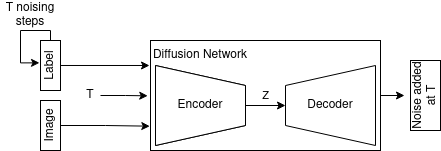
\includegraphics[width=\linewidth]{Diffusion Model}
    \caption{Conditional Diffusion Model}
    \label{fig:DiffusionDiagram}
\end{figure}

% Maybe theres a better way to write this?
% Look at the papers and see if its there
\begin{algorithm}
\caption{Diffusion Model Training Strategy}\label{ALG:Diffusion}
\begin{algorithmic}[1]
\For{$\texttt{every epoch}$}
\For{$I, L \texttt{ in training dataloader}$}
\State
\State $t = random(0, noise\_steps)$
\State $noise_{real}, L_{noisy} = noise\_image(L, t)$ \Comment{Apply t steps of noise}
\State
\State $input = concatenation(I, L_{noisy})$
\State $noise_{pred} = model(input, t)$
\State $loss = MSE( noise_{pred}, Noise_{real} )$
\State $\texttt{Update weights of model with backpropagation}$
\EndFor
\EndFor
\end{algorithmic}
\end{algorithm}

\textbf{Implementation considerations}

C++ and Python are both suitable for machine learning tasks, they both have a plethora of libraries such as TensorFlow, PyTorch, and Caffe that aid in development. In fact, quite a lot of libraries, including the former two, are available on both Python and C++. I have chosen to use Python for this project as, personally, it is the easier language of the two to work with. This project is meant as a proof of concept, and as such I prioritise the quicker development time with Python, over the faster execution speed of C++. I have also chosen to use the PyTorch library to do the majority of the machine learning code, this is because it has lots of prebuilt C++ functions which should speed up execution time significantly. The methods that I will apply should work in any language or framework, PyTorch is simply an abstraction that should shorten development time. I will implement my own UNet code but for the GAN and diffusion models I have chosen to adapt and use code available in the following repositories \cite{PytorchPix2Pix, JanspiryPalette} respectively. Both have licenses that allow their use in this project. 

\textbf{Results Analysis/Testing}
% Maybe theres more to put here?
After training all three models I will compare them using the requirements defined in \ref{tab:RequirementCaptureTable}.

\chapter{Implementation and Experimental Results}

In this chapter I describe the implementation, tuning, and results of my models, how successful they were, and show data about their training.

% INTRODUCE THIS CHAPTER

% Approx 10-15 pages

% add plots and tables of results and explain them
% important facts in text
% compare loss functions
% explain dataset limitations
%    solved with gan
%    in experiments?

\textbf{Experimental Environment}

This model was trained on a computer using an RTX 3070 with 8GB of VRAM and an AMD Ryzen 3600 with 32GB of system RAM, due to the relatively low video RAM a lot of effort was made to keep memory usage down in each model. During training I resized each image to 128px x 128px and after each training epoch explicitly deleted the image, label, and output from memory.
Testing the hyperparameter options for the UNet Autoencoder model took approximately 2 days and I trained the final model over the course of 40 minutes.
Testing the hyperparameter options for GAN model took approximately 3 days and I trained my final model over the course of 2 hours.  
Testing the hyperparameter options for Diffusion model took approximately 2 weeks and I trained the final model over the course of Y hours (Not trained final model yet)
% FILL IN X AND Y

\textbf{Hyperparameter tuning}

When tuning the UNet autoencoder and GAN models I automated the process of exploring the parameter and hyperparameter search space. In my search I varied the following parameters: The normalisation layer used, the channel layouts used, the optimiser used, the learning rates for the optimiser, and, if the Adam optimiser was used, the beta values. In experiment 2 I allowed for the generator and discriminator models to use different normalisation functions, optimisers, and learning rates. 

Training a diffusion model is far more computationally expensive than an autoencoder or a GAN, training and evaluating a GAN model on the VISCHEMA dataset typically took around 200 minutes, where as a diffusion model typically took around 20 hours. 
Because of this I limited my search across diffusion models to manually vary the following parameters of the palette model available at \cite{JanspiryPalette}: the number of channels used, the normalisation layer used, the noise scheduling algorithm, and the number of noise steps.

Exploring these search spaces exhaustively is unfortunately not feasible, for the Autoencoder and GAN models there are over 5000 different possible combinations, and if I tested each combination once for 100 epochs then it would take hundreds of days to test.
Instead I have explored a subset of this search space. For each experiment I estimated default parameter and hyperparameter values, by varying these values I lowered the scope of the search space to approximately 100 permutations. This took \(\sim\)2/3 days per experiment to test. Unfortunately this does mean that not every combination has been tested, however we should achieve a good approximation of the best parameters and hyperparameters.

\textbf{UNet Autoencoder Training and Results}

In this experiment I created and trained a UNet model as described in \cite{ronneberger2015unet} to directly predict the VMS maps of images, I trained the model using backpropagation of the L1 loss, described in equation \ref{eqn:UNet Loss}, of the model output given an image, and the corresponding label. The best parameters and hyperparameters that I found for my model were the following: Encoder Channels = (3,64,128,256,512,1024), Decoder Channels = (1024,512,256,128,64), Batch Normalisation, Adam Optimizer with a learning rate of 0.001 and betas = (0.9, 0.999). A diagram of the training curve for the autoencoder can be seen in figure \ref{fig:autoencoderTraining}. After 80 training epochs I was able to achieve an L1 loss across the validation dataset of ~0.132. A sample of the best output images can be seen in figure \ref{fig:autoencoderBestOutput}, and a sample of the lowest accuracy output images can be seen in figure \ref{fig:autoencoderWorstOutput}. As you can see the autoencoder tends to turn the blocky VMS shape into a rounded circle. It is less accurately able predict the red regions, this is likely due to there being far more green data than red data.

\textbf{UNet Autoencoder Requirements Fit}
As outlined in \ref{tab:RequirementCaptureTable} our best autoencoder model succeeded in the following requirements: 1.1 as it is possible to input an image, 1.2 as the model produces an image when given an input, 1.3 as the mean output loss is relatively low, and 2.1 as it is able to produce an image fast, in approximately 7 milliseconds.
Unfortunately when I qualitatively analyse the images the model does not succeed in achieving requirement 1.4, it learns a somewhat accurate mapping but typically smooth out the blocky VMS components into circular shapes. There are also clear small visual blotches present in all of the predictions, these do not seem to line up with anything in particular in the input image or label.   

\begin{figure}[ht]
    \centering
    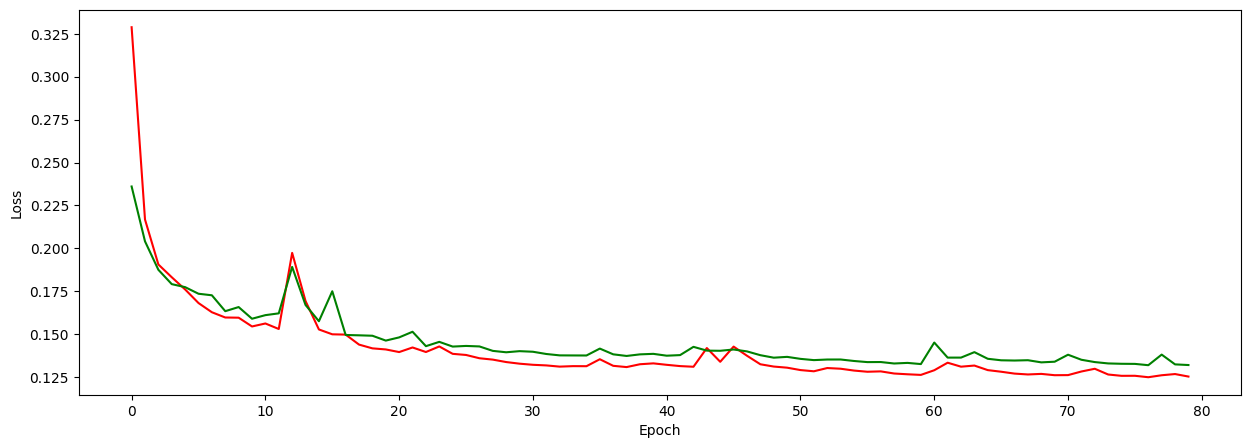
\includegraphics[width=\linewidth]{Autoencoder Training Curve}
    \caption{Autoencoder training graph. The red plot describes the training loss per epoch and the green plot the validation loss. The validation loss closely matches the training loss, indicating that the model does not become overfit to the training data.}
    \label{fig:autoencoderTraining}
\end{figure}

\begin{figure}[ht]
    \centering
    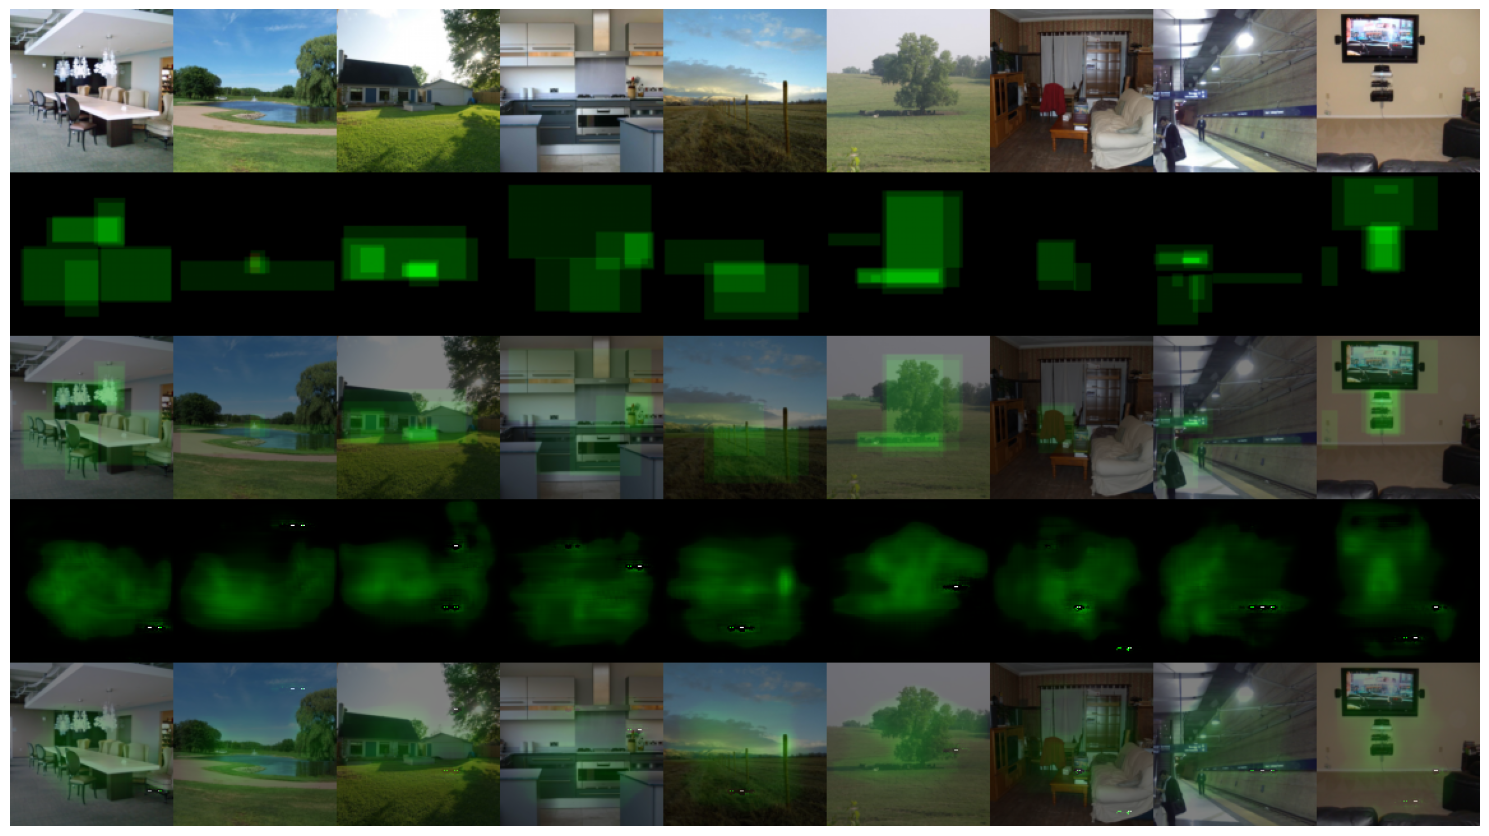
\includegraphics[width=\linewidth]{Best autoencoder Outputs}
    \caption{Best Autoencoder Outputs}
    \label{fig:autoencoderBestOutput}
\end{figure}

\textbf{GAN Training and Results}

% https://github.com/junyanz/pytorch-CycleGAN-and-pix2pix/issues/1081
This experiment was performed with differentiable augmentation as described in \cite{zhao2020differentiable}. I performed translation and cutout, each with a 90\% chance.

After performing a hyperparameter search, training each model for approximately 100 epochs, we find that the best hyperparameters for our Generator and Discriminator are as follows:

\textbf{Best Generator}: Batch normalisation, Encoder channel layout = (6, 64, 128, 256, 512, 1024), Decoder channel layout = (1024, 512, 256, 128, 64, 3), Adam optimiser with betas = (0.5, 0.999) and an initial learning rate of 0.0002.

\textbf{Best Discriminator}: Batch normalisation, Channel layout = (6, 64, 128, 256, 512), Adam optimiser with betas = (0.5, 0.999) and a learning rate of 0.0002.

Using these parameters, after 200 epochs of training our model is able to achieve a mean L1 score of ~0.0740 across our validation dataset. This is significantly better than our autoencoder model. A diagram of the training curve for the final GAN model can be seen in figure \ref{fig:GANTraining}. 
Figure \ref{fig:GANBestOutput} shows the outputs across the validation portion of our dataset with the lowest L1 Loss. The outputs presented in this figure are accurately labelled with the correct regions as memorable, but frankly are quite boring and do not necessarily show off the high quality outputs capable of our model, the low L1 loss across these is because the labels simply have lots of black data, therefore any model that just predicts fully black images with random green regions would likely have a low loss across these images. 
Instead I present figure \ref{fig:GANGoodOutput} which shows what I think are far more impressive results, despite the higher loss than the images presented in figure \ref{fig:GANBestOutput}. For these images the model is able to accurately predict large regions of the image that are memorable. This is why requirement 1.4 is important, it qualitative analysis allows for a much more nuanced analysis of how the outputs look.  
The worst results are shown in \ref{fig:GANWorstOutput}, it appears that, like our autoencoder model from experiment 1, this model finds it difficult to predict red regions, i.e. those that users hallucinate remembering.

\begin{figure}[ht]
    \centering
    \includegraphics[width=\linewidth]{GAN Training Curve}
    \caption{GAN training graph. There are 4 losses plotted in this graph, in pale green and dark green the L1 loss across and it's linear regression respectively, in blue the loss when tricking the discriminator, in red and orange the discriminator loss when predicting fake and real images respectively.}
    \label{fig:GANTraining}
\end{figure}

\begin{figure}[ht]
    \centering
    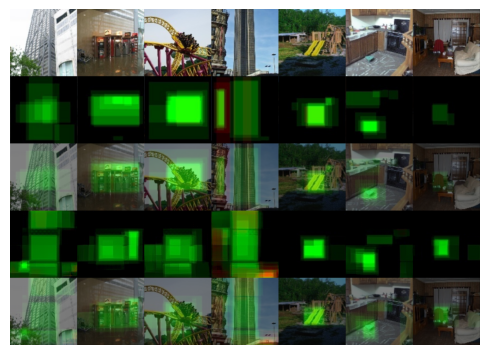
\includegraphics[width=\linewidth]{Good GAN Outputs}
    \caption{Favourite GAN Outputs}
    \label{fig:GANGoodOutput}
\end{figure}

\textbf{GAN Requirements Fit}
Our best GAN model is incredibly successful and achieves all requirements outlined in \ref{tab:RequirementCaptureTable}: 1.1 as it is possible to input an image, 1.2 as the model produces an image when given an input, 1.3 as the mean output loss is very low, 1.4, it learns a very accurate model of the mapping and is able to create convincing memorability maps and 2.1 as it is able to produce an image in ~3.0 milliseconds. My only concern would be that it fails to accurately predict the red component of the VMS images, however I believe this is significantly less important than predicting the green component, and as such our model is still successful.

\textbf{Diffusion Model Training and Results}

I found that the best parameters for this network were: Group Normalisation, Encoder channel layout = (64, 128, 256, 512), Decoder channel layout = (512, 256, 128, 64), and a cosine beta scheduler with a start of 1e-6 and an end of 0.02.

Evaluating the L1 loss of the diffusion models across the entire validation distribution takes approximately 2 hours with the parameters above, because of this, during training I couldn't see if the L1 loss was going down, I could still test if it was overfitting by evaluating the ability to remove a random step of noise every epoch across the validation set. The graph in figure 
\ref{fig:DiffusionTraining}
shows the mean training and validation loss per epoch for my best model, the validation loss in this case is the loss for removing 1 step of noise from each image, not the full 2000. The green plot indicates validation performance, and red training. The plots stay very close together until epoch 350 at which point the model starts to become overfit. This is more obvious in figure \ref{fig:DiffusionTrainingOverfit}, where I show the training curve from epoch 100 onwards. Because of this I have chosen to use early stopping and use the weights of my model at epoch 350.
You can see a selection of the best model predictions in figure 
\ref{fig:DiffusionBestOutputs}
and a selection of the worst model predictions in figure 
\ref{fig:DiffusionWorstOutput}
. As you can see the network still produces images with random noise, unfortunately I could not solve this issue. In this experiment I was only able to explore a small range of possible hyperparameters and as such my results do not emulate the recent success found in diffusion based image generation \cite{ramesh2022hierarchical, saharia2022photorealistic}. However, with a greater number of computing resources, specifically parallel GPUs, it should be possible to explore a greater search space and achieve better results.

\begin{figure}[ht]
    \centering
    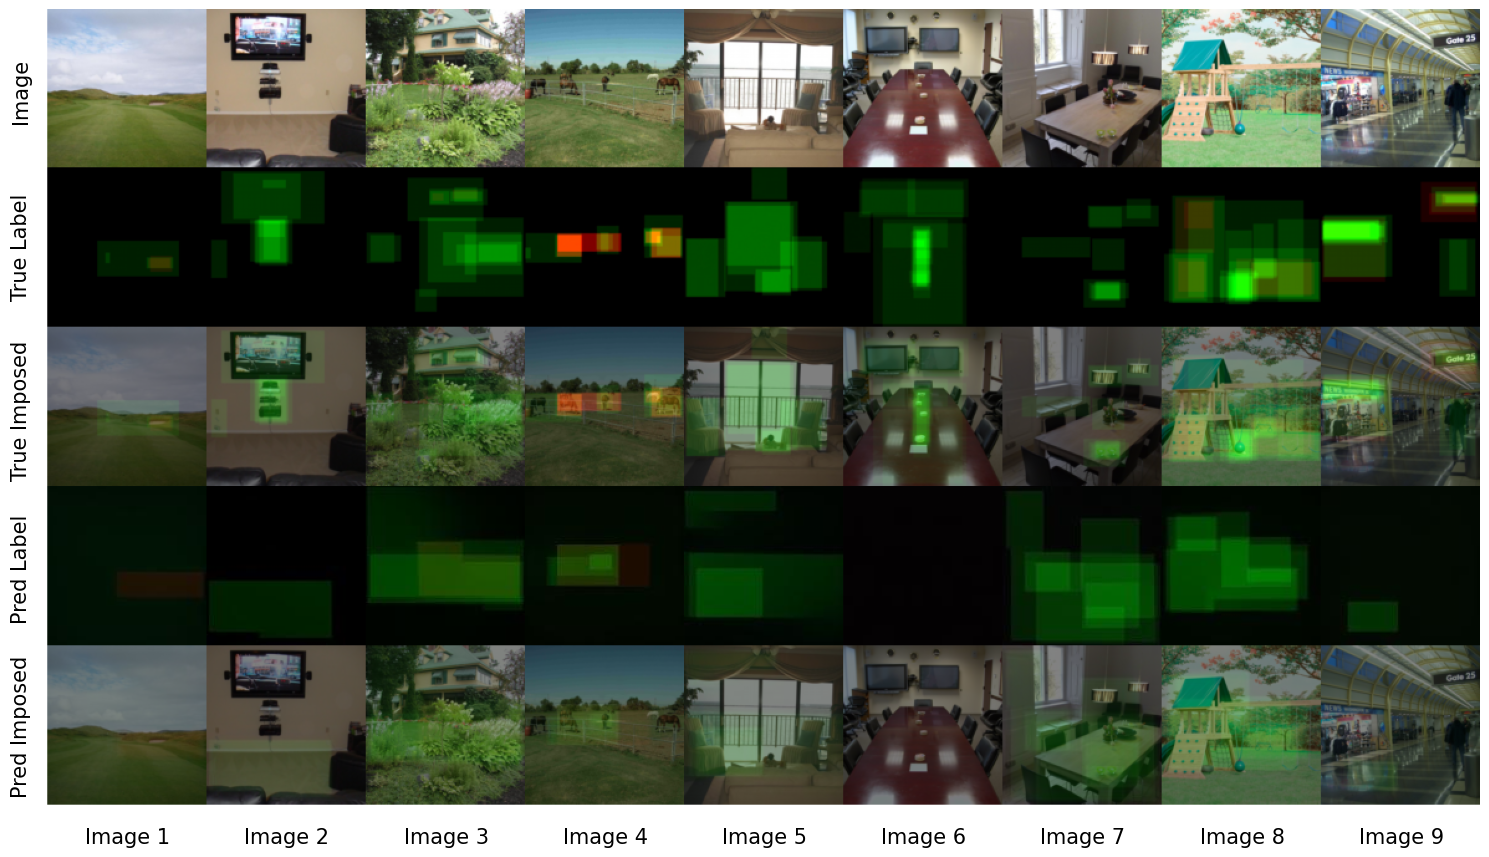
\includegraphics[width=\linewidth]{Diffusion Best Outputs}
    \caption{Best Diffusion Outputs}
    \label{fig:DiffusionBestOutputs}
\end{figure}

\begin{figure}[ht]
    \centering
    \includegraphics[width=\linewidth]{Diffusion training curve}
    \caption{Diffusion Training Curve}
    \label{fig:DiffusionTraining}
\end{figure}

\textbf{Diffusion Requirements Fit}
%Some discussion about them.

My best diffusion model is unfortunately unsuccessful. It is only able to pass requirements 1.1 and 1.2; you can input an image and it outputs an image. The output images have a large mean loss of \( \sim 0.31 \) and as such fail requirement 1.3, and when I qualitatively analyse the output images, they either look like accurate VMS maps for completely different images or look noisy, and as such the model fails requirement 1.4. The model also takes on average 23 seconds to produce an image, this is far too long compared to our autoencoder and GAN models, and as such it fails requirement 2.1. 

\textbf{Examination Across VISCHEMA Categories}

The dataset that I trained on, VISCHEMA PLUS, is composed of two datasets: VISCHEMA and VISCHEMA 2. The VISCHEMA dataset is split into 12 distinct classes, the VISCHEMA 2 dataset is split into 8 distinct classes. The "kitchen" class is present in both datasets, but otherwise classes are exclusive to VISCHEMA or VISCHEMA 2. In figure \ref{tab:categories} the average L1 loss each model achieves across each different class in the validation distribution is displayed. The values are rounded to 2 significant figures but in calculations I used the un-rounded versions. 

Looking at this data we can see that our GAN model is the most consistent, with a standard deviation of the mean L1 loss across the different classes \( \sim 0.022\), the autoencoder model is the least consistent with a standard deviation of \( \sim 0.052\), and our diffusion model is in the middle with a standard deviation of \( \sim 0.047\). Across both our autoencoder and GAN models, the accuracy in measuring memorability maps for skyscrapers is the lowest, this is likely due to the large red regions in the VMS that our model has difficulty predicting, interestingly, this is one of the best classes that our diffusion model produces results for. Looking at the diffusion model outputs I can see that it has a tendency to predict red far more often than the other networks, this may be the reason that it produces much better results for skyscrapers compared to other classes.

% Populated
% Big
% public entertainment
% isolated
% small
% work-home

\begin{table}[ht]
    \centering
    \begin{tabular}{|l|lll|}
        \hline
        \multicolumn{1}{|c|}{} & \multicolumn{3}{c|}{Model}                                                                          \\ \hline
        Category               & \multicolumn{1}{c|}{Autoencoder} & \multicolumn{1}{c|}{GAN}  & \multicolumn{1}{c|}{Diffusion Model} \\ \hline
        Kitchen                & \multicolumn{1}{l|}{0.12}        & \multicolumn{1}{l|}{0.072}& 0.35                                    \\ \hline
        Living Room            & \multicolumn{1}{l|}{0.13}        & \multicolumn{1}{l|}{0.047}& 0.28                                    \\ \hline
        Conf. Room             & \multicolumn{1}{l|}{0.17}        & \multicolumn{1}{l|}{0.091}& 0.34                                    \\ \hline
        Airport Ter.           & \multicolumn{1}{l|}{0.15}        & \multicolumn{1}{l|}{0.085}& 0.29                                    \\ \hline
        House                  & \multicolumn{1}{l|}{0.13}        & \multicolumn{1}{l|}{0.075}& 0.25                                    \\ \hline
        Skyscraper             & \multicolumn{1}{l|}{0.31}        & \multicolumn{1}{l|}{0.14 }& 0.31                                    \\ \hline
        Amus. Park             & \multicolumn{1}{l|}{0.14}        & \multicolumn{1}{l|}{0.086}& 0.44                                    \\ \hline
        Playground             & \multicolumn{1}{l|}{0.14}        & \multicolumn{1}{l|}{0.079}& 0.34                                    \\ \hline
        Pasture                & \multicolumn{1}{l|}{0.11}        & \multicolumn{1}{l|}{0.056}& 0.37                                    \\ \hline
        Golf Course            & \multicolumn{1}{l|}{0.13}        & \multicolumn{1}{l|}{0.076}& 0.34                                    \\ \hline
        Mountain               & \multicolumn{1}{l|}{0.19}        & \multicolumn{1}{l|}{0.094}& 0.32                                    \\ \hline
        Badland                & \multicolumn{1}{l|}{0.20}        & \multicolumn{1}{l|}{0.096}& 0.23                                    \\ \hline
        
        Populated              & \multicolumn{1}{l|}{0.20}        & \multicolumn{1}{l|}{0.0077}& 0.34                                   \\ \hline
        Big                    & \multicolumn{1}{l|}{0.20}        & \multicolumn{1}{l|}{0.014}& 0.29                                    \\ \hline
        Public Ent.            & \multicolumn{1}{l|}{0.20}        & \multicolumn{1}{l|}{0.018}& 0.31                                    \\ \hline
        Isolated               & \multicolumn{1}{l|}{0.20}        & \multicolumn{1}{l|}{0.029}& 0.28                                    \\ \hline
        Small                  & \multicolumn{1}{l|}{0.20}        & \multicolumn{1}{l|}{0.016}& 0.34                                    \\ \hline
        Work-Home              & \multicolumn{1}{l|}{0.20}        & \multicolumn{1}{l|}{0.027}& 0.24                                    \\ \hline
        \hline
        Mean                   & \multicolumn{1}{l|}{0.14}        & \multicolumn{1}{l|}{0.077}& 0.31                                    \\ \hline
        Median                 & \multicolumn{1}{l|}{0.13}        & \multicolumn{1}{l|}{0.075}& 0.31                                    \\ \hline
        Std                    & \multicolumn{1}{l|}{0.052}       & \multicolumn{1}{l|}{0.022}& 0.047                                   \\ \hline
    \end{tabular}
    \label{tab:categories}
    \caption{The average L1 loss that each model achieves over the different categories present in the VISCHEMA validation distribution.}
\end{table}

\textbf{Measuring loss across just the Green channel}

Our models have a lot of trouble predicting the red channel of the VMS maps. The red channel indicates that users thought they remembered the image because of this region, when in reality they had not been shown this image before. If we measure the loss of our models across just the green channel, that is the regions subjects indicated triggered their memory in images that they correctly identified as seeing before, 
then our average L1 loss across the validation dataset decreases from ~0.132 to \(\sim \)0.083 with our autoencoder model, 
from ~0.0740 to \(\sim \) 0.046 in our GAN, 
and increases from \(\sim 0.31 \) to \(\sim 0.54 \) in our diffusion model.
Because this loss is the mean across each pixel, we can compare the them regardless of the change in channel depth. Clearly our autoencoder and GAN models are better at predicting green regions rather than red ones. I suspect that this is due to the much larger amount of green data than red in the dataset. I'm not sure why the diffusion model has learned to predict red more prominently than green. The diffusion loss increasing reinforces my belief that it has a tenancy to predict red more often than it appears.

\chapter{Conclusion}

% % Approx 1-2 pages
% % how it went

%Results are skilfully synthesised to identify a detailed set of clear outcomes for the project, and their potential implications in the context of the topic of study are substantial and robustly argued. 
% Outcomes are evaluated on self-defined success criteria for the project and related back to the original aim and motivation of the project. 
%The Conclusions clearly refer back to the implications of the project relating to the overall motivation.

The goal of this project was to explore state of the art image to image models in the context of generating VMS schemas from the VISCHEMA Plus dataset. I had the most success generating these using a Pix2pix style GAN, achieving a mean L1 loss of \(\sim 0.0740 \) and very convincing memorability maps. I had moderate success using an autoencoder, achieving a mean L1 loss of \(\sim 0.132\) and somewhat unconvincing memorability maps. I had very little success using a diffusion model, achieving a mean L1 loss of \(\sim 0.48 \) and memorability maps that very often just look like noise.

The success found in GAN models has many wide reaching applications, image memorability is an important factor in many creative fields, educators want memorable diagrams, marketing agencies want memorable adverts, musicians want memorable album art, movie and TV producers want memorable scenes. While GAN models can take much longer to train than autoencoder models, during evaluation they execute in very similar times, and as such if any creative professional was to use an automated memorability map generator to aid in their work, I would recommend that a GAN model is used, as the increased quality comes at no hit to performance. In fact, because it takes only milliseconds to execute, I could see an application where a memorability map is generated in real time as people make changes to their images.

Even if it were possible to generate accurate and convincing memorability maps using diffusion models, there is also a great issue with the execution time. Nobody would want to wait almost half a minute for the memorability map to be generated, especially in a process that is supposed to be iterative and fast. For their success, not only would the model accuracy have to be increased, but it would also need to generate the VMS schemas in far fewer noise steps/computing power would need to increase significantly to make up for the increased computation required. 

In future work I would love to spend more time working on diffusion models, I find them fascinating and with the success found in the industry \cite{ramesh2022hierarchical, saharia2022photorealistic} it seems feasible to me to fix the accuracy issues. Ideally I would have access to a multi-GPU architecture in order to speed up the development and testing process.

I would also be interested in exploring the application of memorability to videos, there are far more factors involved including audio, movement, fps, that would greatly increase the complexity of the problem. Research has been done in \cite{HASSON2004, HASSONNeurocinematics, HASSON2008, fMRIPredictions} using fMRI scans to estimate the memorability of video streams using an extension of the memorability game. I would love to expand upon this work.

% UNet Autoencoders are simple to implement and I have found that they produce somewhat successful results, they train very quickly and can create labels in milliseconds, but fail under qualitative analysis. 

% GAN models can be difficult to work with, and lots of research has gone into creating versatile and robust GAN architectures, adapting an existing, successful, model to your needs can reduce development time. Using a modified pix2pix GAN model \cite{isola2018imagetoimage} I was able to generate very accurate VMS maps, maintaining the blocky shape of the regions, and achieving a mean L1 loss of \(\sim 0.0740\). Generally, these models took longer to train than my autoencoder models but given an image they are able to produce an image in a similar time to a UNet autoencoder.

% Diffusion models took the longest to train, and while they can generally produce high quality images \cite{ramesh2022hierarchical, saharia2022photorealistic}, the training loop requires a large amount of computational resources, making it difficult to fine tune in a reasonable time. My best model was able to achieve an L1 loss of (Final Diffusion Loss). Due to computational restraints I was unable to run a large hyperparameter search and my results leave room for improvement.
% %FILL IN FINAL DIFFUSION LOSS

% % %The implications of these findings (what these answers mean)

% I show that using a GAN model we are able to predict memorable image regions with great accuracy. I believe this has many useful applications across many different industries, allowing creators to have a more informed opinion on which sections of their images are memorable, using this tool to iteratively improve their image memorability.
% % future work better generator better result

% % applications
% Hopefully in future work good parameters can be found that allow diffusion models to work with lower noise steps and to produce higher accuracy results. Diffusion models lend themselves well to multiple GPU architectures, and if I were to run this project again I would hope to have access to a system capable of running them faster. While diffusion models have seen lots of mainstream attention recently, until home computing power is significantly greater it is infeasible for most to train their own in any reasonable amount of time. 

\chapter{Appendix}

\begin{figure}[ht]
    \centering
    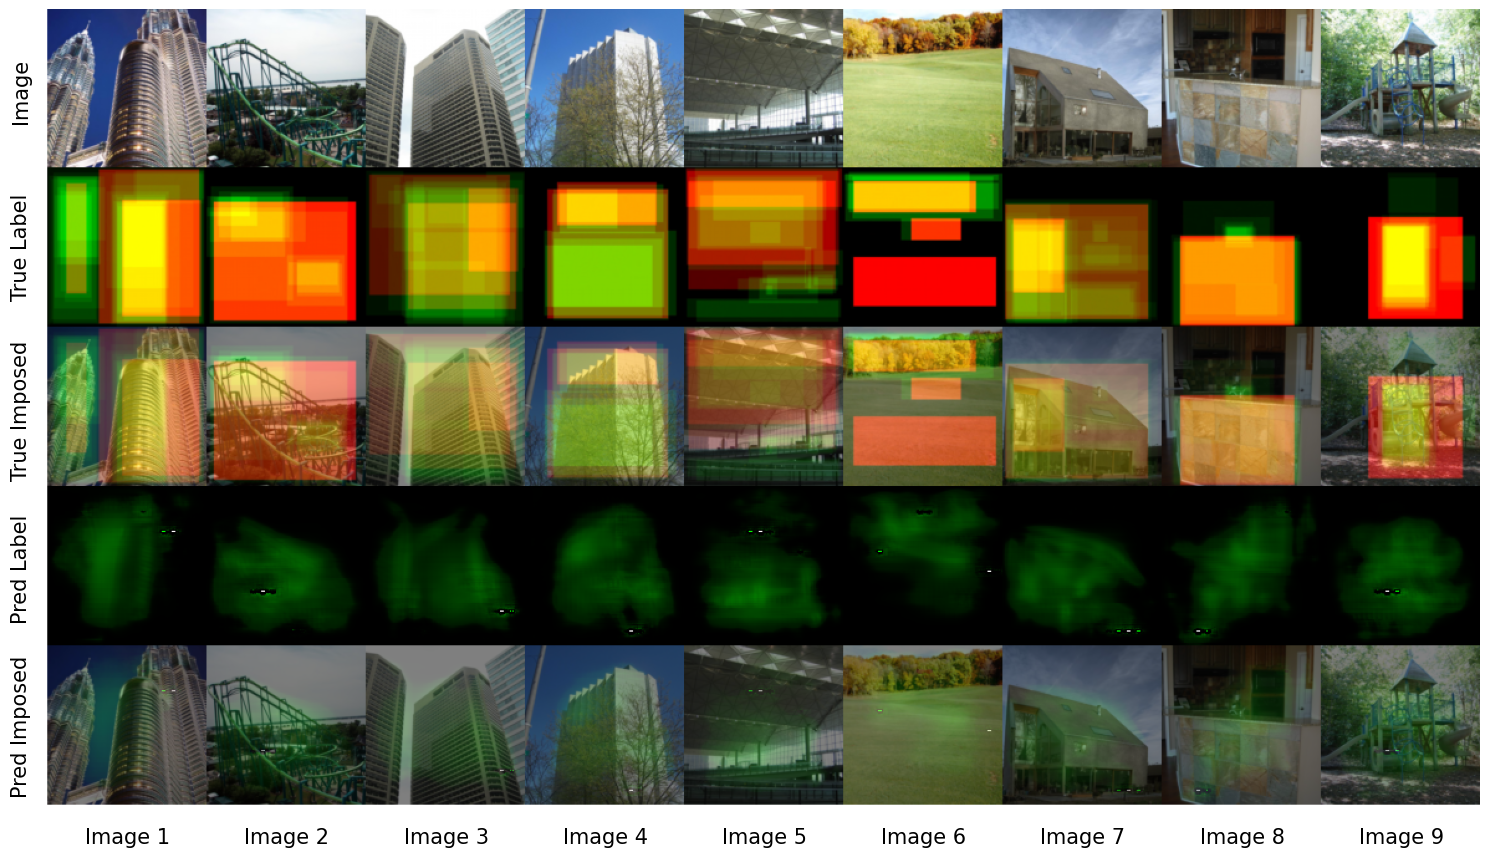
\includegraphics[width=\linewidth]{Worst autoencoder Outputs}
    \caption{Worst Autoencoder Outputs}
    \label{fig:autoencoderWorstOutput}
\end{figure}

\begin{figure}[ht]
    \centering
    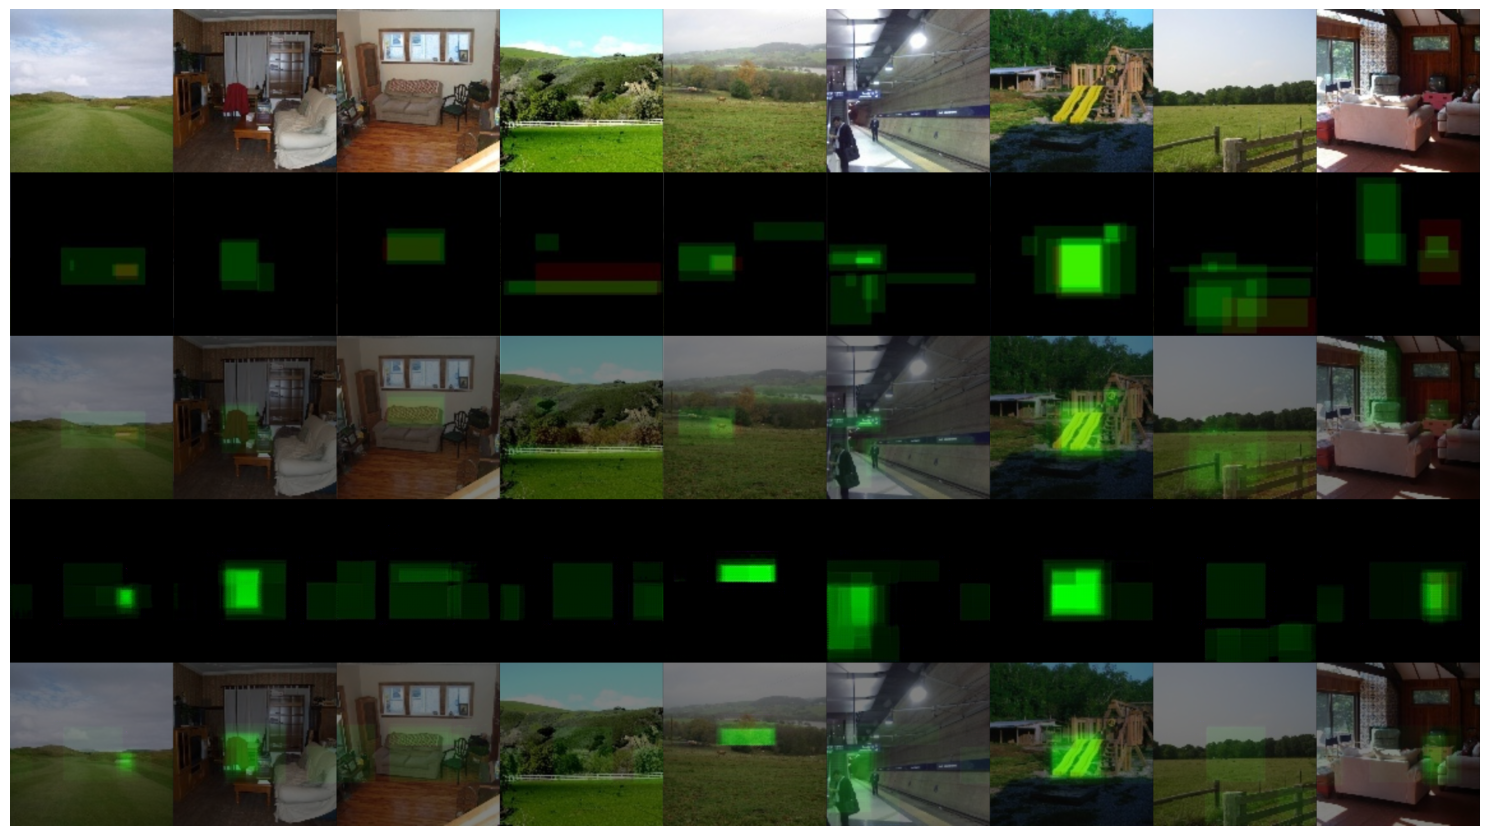
\includegraphics[width=\linewidth]{Best GAN Outputs}
    \caption{Best GAN Outputs}
    \label{fig:GANBestOutput}
\end{figure}

\begin{figure}[ht]
    \centering
    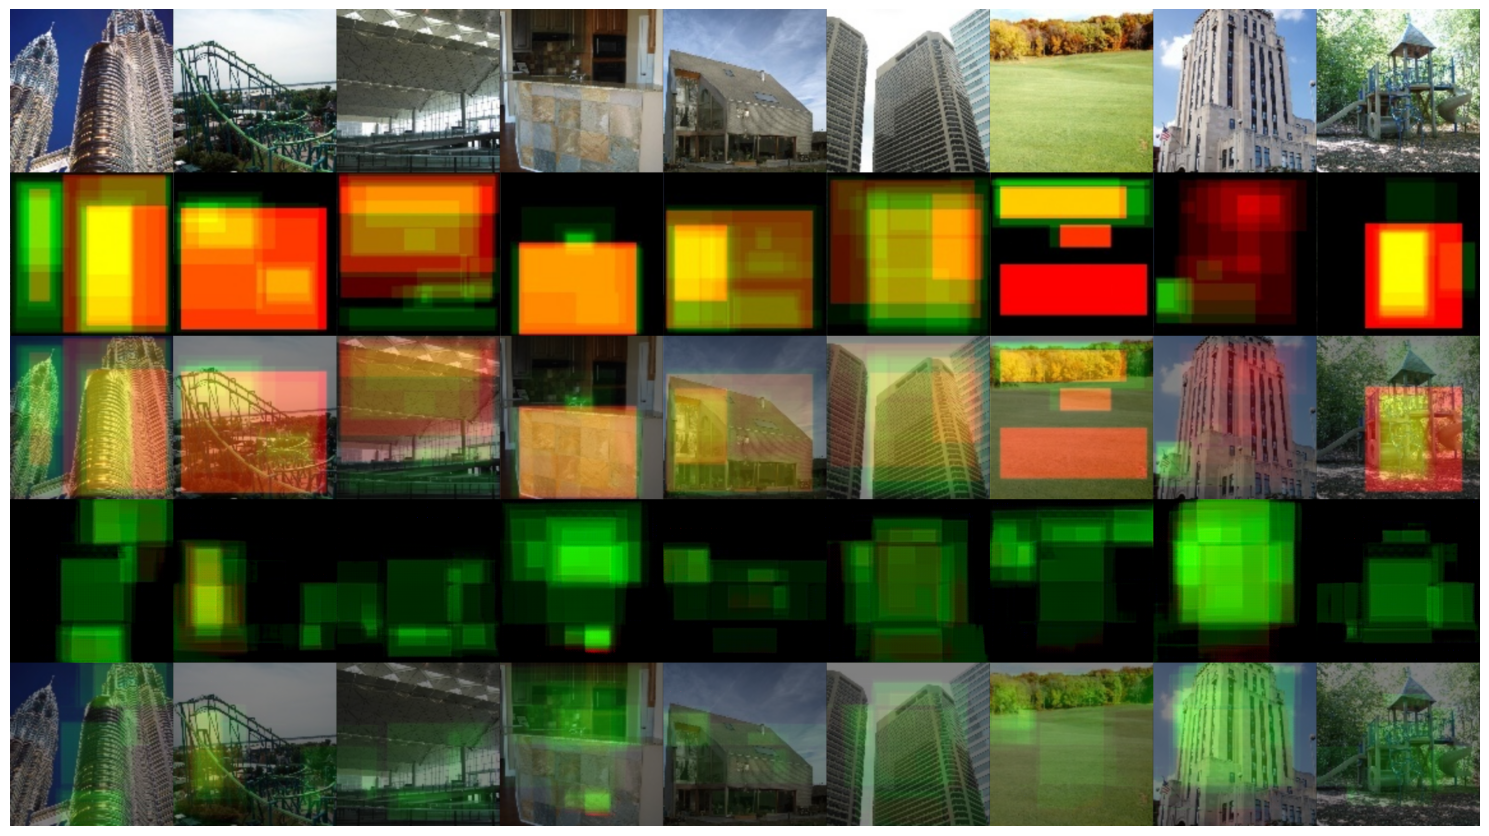
\includegraphics[width=\linewidth]{Worst GAN Outputs}
    \caption{Worst GAN Outputs}
    \label{fig:GANWorstOutput}
\end{figure}

\begin{figure}[ht]
    \centering
    \includegraphics[width=\linewidth]{Diffusion training curve overfit}
    \caption{Diffusion Training Curve from epoch 100 onwards.}
    \label{fig:DiffusionTrainingOverfit}
\end{figure}

\begin{figure}[ht]
    \centering
    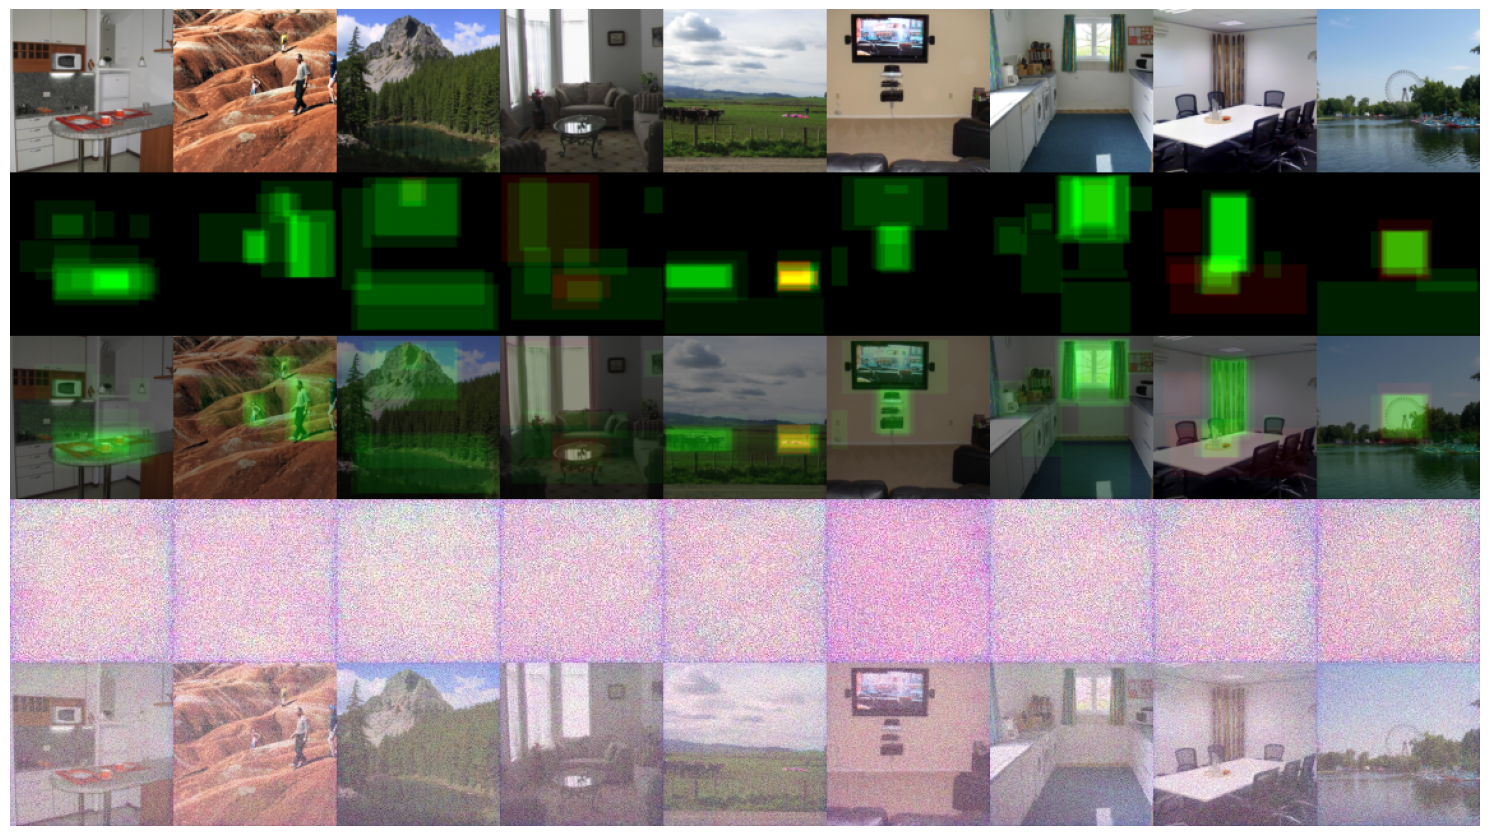
\includegraphics[width=\linewidth]{Worst Diffusion Outputs}
    \caption{Worst Diffusion Outputs}
    \label{fig:DiffusionWorstOutput}
\end{figure}

\printbibliography

\end{document}
